\let\negmpace\undefined
\let\negthickspace\undefined
\documentclass[journal]{IEEEtran}
\usepackage[a5paper, margin=10mm, onecolumn]{geometry}
%\usepackage{lmodern} % Ensure lmodern is loaded for pdflatex
\usepackage{tfrupee} % Include tfrupee package
\setlength{\headheight}{1cm} % Set the height of the header box
\setlength{\headsep}{0mm}     % Set the distance between the header box and the top of the text
\usepackage{xparse}
\usepackage{gvv-book}
\usepackage{gvv}
\usepackage{cite}
\usepackage{amsmath,amssymb,amsfonts,amsthm}
\usepackage{algorithmic}
\usepackage{graphicx}
\usepackage{textcomp}
\usepackage{xcolor}
\usepackage{txfonts}
\usepackage{listings}
\usepackage{enumitem}
\usepackage{mathtools}
\usepackage{gensymb}
\usepackage{comment}
\usepackage[breaklinks=true]{hyperref}
\usepackage{tkz-euclide} 
\usepackage{listings}
% \usepackage{gvv}                                        
\def\inputGnumericTable{}                                 
\usepackage[latin1]{inputenc}                                
\usepackage{color}                                            
\usepackage{array}                                            
\usepackage{longtable}                                       
\usepackage{calc}                                             
\usepackage{multirow}                                         
\usepackage{hhline}                                           
\usepackage{ifthen}                                           
\usepackage{lscape}
\renewcommand{\thefigure}{\theenumi}
\renewcommand{\thetable}{\theenumi}
\setlength{\intextsep}{10pt} % Space between text and floats
\numberwithin{equation}{enumi}
\numberwithin{figure}{enumi}
\renewcommand{\thetable}{\theenumi}
\begin{document}
\bibliographystyle{IEEEtran}
\title{Question-9.7.9}
\author{EE24BTECH11038 - MALAKALA BALA SUBRAHMANYA ARAVIND}
% \maketitle
% \newpage
% \bigskip
{\let\newpage\relax\maketitle}
\textbf{Question}:
Find the particular solution of the differential equation $\brak{1+e^{2x}}$dy+$\brak{1+y^2}e^x$dx=0,given that y=1 and when x=0 \\

\solution \\

The equation can de written as 
\begin{align}
    \frac{dy}{dx}&=-\frac{\brak{1+y^2}e^x}{1+e^{2x}}
\end{align}
This is a first-order, separable differential equation.
\begin{align}
    \frac{1}{1+y^2}\,\,dy&=-\frac{e^x}{1+e^{2x}}\,\,dx
\end{align}
The integral of $\frac{1}{1+y^2}$ is $\tan^{-1}y$\\
The integral of $ \int -\frac{e^x}{1+e^{2x}}\,\,dx$ can be computed as shown below\\
\begin{align}
    \text{Let}\,\,\,\,e^{x}&=t\\
    e^x\,\,dx&=dt\\
    \int -\frac{e^x}{1+e^{2x}}\,\,dx &= \int -\frac{1}{1+t^2}\,\,dt\\
    \int -\frac{1}{1+t^2}\,\,dt&=-\tan^{-1}t\\
    \int -\frac{e^x}{1+e^{2x}}\,\,dx&=-\tan^{-1}{e^x}
\end{align}
The final solution is 
\begin{align}
    \tan^{-1}y&=\tan^{-1}{e^x}+c
\end{align}
At x=0 the value of y is 1 on substituting
\begin{align}
    \tan^{-1}{1}=-\tan^{-1}{e^0}+c\\
    \frac{\pi}{4}=-\frac{\pi}{4}+c\\
    c=\frac{\pi}{2}
\end{align}
The final solution is 
\begin{align}
    \tan^{-1}{y}=-\tan^{-1}{e^x}+\frac{\pi}{2}
\end{align}
\noindent\textbf{Numerical Approach:}\\1. I used a for loop for finding the $y$ values as the loop proceeds with iterative formula given below. I took some initial value of $x$ and as loop proceeds I assigned it the value as $x+h$. where $h$ is the step size, representing the rate of change. 
\\2. Assigned the values of $y$ for different $x$-values using a for loop. \\ 
\\ \textbf{Using the Method of Finite Differences}\\
The Method of Finite Differences is a numerical technique used to approximate solutions to differential equations. 

We know that:
\begin{align}
   \lim_{h \to 0} \frac{y(x+h) - y(x)}{h} &= \frac{dy}{dx} 
\end{align}
For the given differential equation,
\begin{align}
    \frac{dy}{dx}&=-\frac{\brak{1+y^2}e^x}{1+e^{2x}}\\
    \frac{y_{n+1} - y_n}{h}&\approx -\frac{\brak{1+y_n^2}e^x_n}{1+e^{2x_n}} \\
    y_{n+1} &= y_n + h \cdot \-\frac{\brak{1+y_n^2}e^x_n}{1+e^{2x_n}}
\end{align}
The iterative formula for updating $x$-values is: 
\begin{align}
    x_n=x_{n-1}+h
\end{align}    
Using Matplotlib, I plotted the computed points and the graph of the exact solution to verify that they approximately match
\begin{figure}[h!]
	\centering
	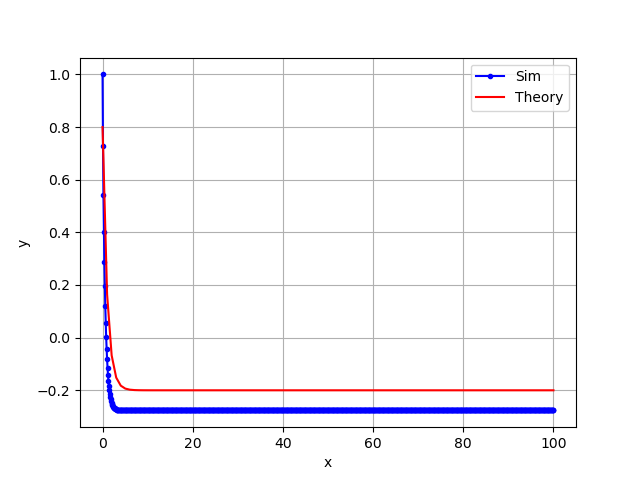
\includegraphics[width=\columnwidth]{figs/Figure_1.png}
	\label{stemplot}
\end{figure}
\end{document}
